The thesis will utilize a design research methodology to perform its research. 
The guidelines provided in \citet{Hevner2004} will be followed to ensure that the process is rigorous.
The guidelines provided in this article are:
\begin{enumerate}
    \item \label{gl1}Design as an Artifact
    \item \label{gl2}Problem Relevance
    \item \label{gl3}Design Evaluation
    \item \label{gl4}Research Contributions
    \item \label{gl5}Research Rigor
    \item \label{gl6}Design as a Search Process
    \item \label{gl7}Communication of Research
\end{enumerate}

We will now explain how we intend to follow these guidelines in our project.
The first guideline says that a design research project should produce some artefact. For this project the artefact is \theartefact. 

The second guideline is justified in section \ref{sec:Research}, and has to do with the objective of a design research project. 
The goal as stated here should be to develop an artefact that is relevant for solving some business problem.

Design evaluation is also mentioned and this guideline stresses the need for rigorous evaluation of the artefact that has been developed.
There are several metrics that are possible for \theartefact, but we will focus on ease of use, and quality of the data.

The research contribution of this project will be \theartefact, which will contribute to solve the problem of how to get users to create semantic content, and how to create open user created knowledge bases for POI data.

The need for research rigor, which is mentioned in guideline \ref{gl5} will be followed by following the multimethodological approach suggested in \citet{Chen1990} and \citet{NunamakerJr1990}. 
This will be the topic of the following section.

Guideline \ref{gl6} says that design research should be a search process. 
In this context that means that one should explore the possible implementations of the artefact by iterating through phases of generating prototypes and testing these prototypes against the requirements of the project( as seen in figure \ref{GenerateTestCycle}, page \pageref{GenerateTestCycle}).
To attain this type of cycle we will chose a system development methodology which utilizes multiple iterations of building and testing.
The last guideline proposed has to do with clear communication of the results of the research. 
It is further proposed that one should take care to have several channels of communication with different levels of technical detail.
The reasoning is that we need to convince both the technical and the managerial communities. 

To conform to the seventh guideline one should communicate the results of ones research in such a way that it is accessible for the intended target audience.
For this thesis, the written thesis itself will be the technical document, documenting the process of designing and implementing the artefact, focusing on an academic audience.
The document talking to management will take the form of a presentation highlighting the benefits of a user generated knowledge base, and the potential business uses.

\begin{figure}[h]
    \begin{center}
        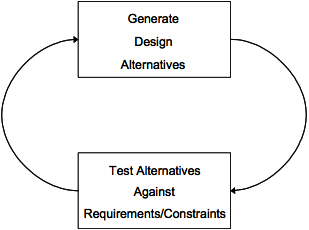
\includegraphics[width=0.60\textwidth]{Images/GenerateTestCycle.png}
        \caption{The generate/test cycle, from \protect \citet{Hevner2004}}
        \label{GenerateTestCycle}
    \end{center}
\end{figure}

For the design process we look to \citet{Chen1990}, who proposes four activities that interact in the development of information systems( See figure \ref{multi} on page \pageref{multi}). 
The paper suggests using a multimethodological approach where one moves between different research activities: Theory building, experimentation, observation and systems development.
By using these different approaches we can hope that we will catch important facets that might otherwise have been missed or over looked.   

\begin{figure}[h]
    \begin{center}
        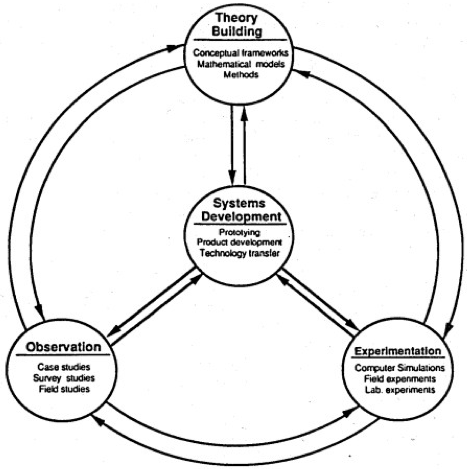
\includegraphics[width=0.60\textwidth]{Images/MultiMethodological.png}
        \caption{A multimethodological approach to IS research, from \protect \citet{Chen1990}}
        \label{multi}
    \end{center}
\end{figure}

% \citet{NunamakerJr1990} The article without the model
\subsection{Experimentation}
There are going to be three main experimentation phases in the thesis.
Before the main part of development starts we will look at how users want use tags to describe POIs.
During development we will periodically perform small usability tests to ensure that development is going the right way.
At the end of development we will also perform a larger user test, both to get data on the final product, and to more accurately judge how good the data created is.

To find out how we are going to design the artefact, we should get some data about how people tag.
To get this data we will perform an experiment on an early prototype of the system, with just the ability to add tags to describe a POI. 
The prototype could be a simple web interface with an input field, or could be as simple a notepad and a pen.
The choice of using a web interface or pen and paper would have to do with a cost benefit analysis, 
with the cost of creating the web prototype against the added validity of having an interface which is closer to the one the finished artifact will have.
Either way, this prototype will be used to perform experiments on the potential user groups. 

The experiment would consist of having a set of POIs that the subjects would be prompted to add information about. 
The subjects should be prompted beforehand to consider that they were adding tags that should help travelers find places they are interested inn, so they know the context of the tags.
These results can be analysed to see if there is a trend in the type of tags that were used. 
The results might help us find out what kind of framing we need for the artefact to get users to add the type of information we are interested in.

The usability studies performed during development will be performed periodically on small groups.
To keep these tests manageable we are going to use small test groups (3-4 users).
Using small test groups like this has been suggested by \citet{Nilsen2000}, and is somewhat backed by \citet{Bevan2003}. 
The claim made is that small user groups are enough to uncover problems with the artefact and that large groups are not needed
since the objective is to uncover pit falls, not to prove theories empirically.

At the end of development there will be a larger usability test to see if the artefact is simple enough in use that
users can express the things they want, and powerful enough to create RDF data of such a high quality that it can be reasoned about.


\subsection{Observation}
We are also going to carry out some observation of how people use tags to describe POIs on the web, 
and what type of information people want when they are planning to travel to a new location.
For both methods we are going to select a few POIs in Bergen, and see both what kind of information people want when they come to visit Bergen,
and what information they think to add about the POIs.
The POIs selected should be picked from different categories like stores, landmarks, restaurants, and hotels to capture a broad selection possible targets.
We want to use commercial POIs as well as non-commercial, even though it might be more difficult to find user generated tags for these.
The reason for this is that to create a successful data store for tourism, we also need information about commercial POIs, as these are of interest for travelers.
Using the same POIs for both tests will make comparing the results easier. 
Therefore we will stive to find commercial POIs that are taged.
We will use two different methods to get this information.

We will look at how people actually use tags to talk about and describe POIs on the internet now by looking at web sites that allows users to add tags. 
To do this we will implement a simple web crawler that picks up tags about the selected POIs.
Flickr\footnote{\url{http://www.flickr.com/}}, and Delicious\footnote{\url{http://delicious.com/}} are obvious places to start, 
but more research could be done to find better or additional sources before the observation begins.
Seeing that the internet is a virtual, not a physical, space, this type of observation is a close approximation of a field study, one of the methods suggested by \citet{Chen1990}.
The idea of analyzing data for finding interesting data for an ontology from Flicker tags was also explored by \citet{Schmitz2006}. 
In that article the attempt was to build an ontology by analyzing the co-occurrence of tags on Flickr as a whole. 
We will instead look at what type of tags people use, and their frequency of use.
This route has the advantage of being routed in the current use of tags. 

There would also be a large data set available, making it possible to potentially make strong statements about how tags are used to describe content.
Creating data sets for a set number of POIs can also be done simply through the sites APIs.
The disadvantage of this approach is that this would be a measure of how people use tags now. 
Depending on how one conceptualize, frame and present the artifact it is possible that the users would use tags differently in our system.

If we find that the current use if close to the one that we want to use in our artefact, 
or if we find that the type of tag used if platform dependent, 
then this will be an indication that setting a context for tagging might be enough.
If not then we might have to look into how we can convince users to tag differently when using our artefact.


We will also use surveys, one of the observational methodologies mentioned by \citet{Chen1990}, to gather information about what type of information users want about POIs.
The plan is to create a survey which mentions the POIs selected in Bergen, and which asks the subject what kind of information about these POIs they would want. 
The survey should contain open ended questions as to get the whole width of possible information that is wanted.
The survey will target tourists in Bergen. 
These could be targeted by for example going to the tourist information agency, and asking the people who are there if they would like to participate.
As with the usability studies, the sample size does not have to be large enough to enable us to make statistically significant statements,
but they should be large enough to give us an insight into what kind of information tourists want about POIs. 
A sample size of 10-20 subjects should be sufficient.
 
Using the data from these three sources should give us ample information about how tags are used currently used to describe POIs, 
how subjects tag POIs when they are aware that they are tagging in the context of helping travelers, 
and what information people want when they think about traveling. 

The data gathered here will also be used to create the final success criteria for the artefact. 
The artefact will be successful if it can provide the types of data that users would want. 
The activities in this part should be seen in light of \citet{Chen1990} as research activities. 
Both the survey and looking at tag usage on the web are instances of observational studies.


\subsection{System development}
To ensure that the system development process is done in a reliable way we should find some structured process to try to follow.
For this project we are going to use a methodology called personal scrum, which is described by \citet{Pruitt2011}.
Personal scrum is a variation of SCRUM as introduced by \citet{Schwaber1995}. 
The main difference that SCRUM focuses on groups and group activities, while personal scrum is a variant with guidelines for how to do a SCRUM like methodology with a one person team.

The reason for choosing this methodology is that SCRUM is a time proven and popular methodology, with a strong emphasis on time boxing and incremental design.
To help the incremental design the requirements for the projects are translated into user stories,
short stories that says something about what users of the system should experience when using the system.
The methodology divides the development process into smaller chunks called sprints. 
A sprint consists of a set of user stories that the team commits to completed before the end of the sprint.
The set of user stories chosen for a sprint are the ones that are deemed the most critical, and which are not dependent on later stories. 
Each sprint finish with a new iteration of a complete product, which can be tested by a user group.
The fact that the methodology uses small sprints which ends with testable products make it a suitable choice.
We could for example switch between system development and experimentation or user testing, two of the activities in figure \ref{multi}.
We could also try out different representations of tags suggested in the literature \citep{Mika2005,Gruber2007,Scerri2008}, 
switching between developing the artefact and commenting on and expanding the literature.

\subsubsection{Initial spike}
Before development of the artefact can start we need to learn the tools we will be using. 
The main part of this phase will be exploring the API exposed by lexitags, and to get to know how to use the different methods.
Since a large part of the system will rely on interaction with lexitags, it is important to know the workings of the tool before designing the artefact.

\subsection{Theory building}
The theory building in the development of \theartefact\ will mainly consist of the evaluation of the artefact at the end.
After the final iteration we will be able to test the artefact against the requirements found in our surveys, 
and see if we are able to generate the type of information we want, and if the information is of a high enough quality.
At this point we will draw in data from all the activities to form a coherent theory.

Before this we might have to look at the theory for representing tags.
By examining and testing the models through development we can se if any of the current models are suitable for our artefact.
If this examination finds that none of the models are suitable for this kind of artefact, we might have to stop development
until such a model can be conceptualized.







